\documentclass[onecolumn,11pt]{report}
%*********
%Paquetes
%*********
\usepackage[spanish]{babel}
\usepackage[utf8]{inputenc}
\usepackage[a4paper, total={7in, 9in}]{geometry}
\usepackage{amsfonts}
\usepackage{dsfont}
\usepackage{physics}
\usepackage{xcolor}
\usepackage{tikz-cd} %para diagrama conmutatitvo
\usepackage{multicol} %para la lista de operadores
\usepackage{hyperref}
\usepackage{caption}
\usepackage{subcaption}


%*********
%Comandos
%*********
\newcommand{\mcU}{\mathcal{U}}
\newcommand{\mcV}{\mathcal{V}}
\newcommand{\mcO}{\mathcal{O}}
\newcommand{\mcI}{\mathcal{I}}
\newcommand{\mcL}{\mathcal{L}}
\newcommand{\mcS}{\mathcal{S}}
\newcommand{\hilbert}{{\sf H}}
\newcommand{\mcB}{\mathcal{B}}
\newcommand{\mcH}{\mathcal{H}}
\newcommand{\mcF}{\mathcal{F}}
\newcommand{\mcC}{\mathcal{C}}
\newcommand{\mcT}{\mathcal{T}}
\newcommand{\mcE}{\ensuremath{\mathcal{E}} }
\newcommand{\mcG}{\ensuremath{\mathcal{G}} }
\newcommand{\mcM}{\mathcal{M}}
\newcommand{\mcN}{\mathcal{N}}
\newcommand{\nnn}{\mathcal{N}}
\newcommand{\choi}{\ensuremath{\mcD} }
\newcommand{\mmm}{\mathcal{M}}
\newcommand{\sss}{\mathcal{S}}
\newcommand{\mcD}{\mathcal{D}}
\newcommand{\mcA}{\mathcal{A}}
\newcommand{\mcP}{\mathcal{P}}
\newcommand{\Complex}{\mathbb{C}} %Para escribir al espacio de hilbert complejo
\newcommand{\Id}{\mathds{1}}% Para escribir el op. indentidad con notación chida
\newcommand{\CG}[1]{\mcC\left[#1\right]}
\newcommand{\Fuzzy}[1]{\mcF\left[#1\right]}
\newcommand{\nota}[1]{{\color{red} [#1]}}
\newcommand{\notaAd}[1]{{\color{blue} [#1]}} %Notas pero mías



\title{Dinámica de un sistema de dos qubits bajo un modelo de grano grueso}
\author{Adán Castillo Guerrero}
\date{\today}

\begin{document}

\maketitle
\begin{abstract}
    Esta bitácora deberá ayudarme a mantener una mejor organización de los resultados conforme los voy obteniendo. \cite{Chuang}
\end{abstract}
\tableofcontents
\newpage
\chapter{Resultados generales}

\section{Diferentes formas de abordar la dinámica}
El objetivo de la tesis es contruir y estudiar ``dinámicas gruesas'', $\Gamma_t$,
\begin{align*}
\Gamma_{t}:&\mcS(\hilbert_2)\rightarrow \mcS(\hilbert_2)\\
&\rho(0) \mapsto \rho(t).
\end{align*}
La dinámica gruesa puede verse como una composición
\begin{equation*}
\Gamma_t:=\mcC \circ \mcU_t \circ \mcA_\mcC.
\end{equation*}
ilustrable a través del siguiente diagrama
\[\begin{tikzcd}[arrows={<-|}]
\rho(0)  & \rho(t) \arrow{l}{\Gamma_{t}} \arrow{d}{\mcC}\\
\varrho(0) \arrow{u}{\mcA_{\mcC}} & \varrho(t). \arrow{l}{\mcU_{t}}
\end{tikzcd}
\]
Si la evolución subyacente total es una operación unitaria $\mcU$, entonces $\mcU_{t}$  denota exactamente $\mcU^{t}$. De esta forma, $\mcU_{t=0}=\Id$, mientras que  $\mcU_{t=1}=\mcU$. De esta forma es que se introduce la dependencia de la variable temporal en $\rho$:
\begin{equation*}
\rho(t)=(\mcC \circ \mcU_t \circ \mcA_\mcC)\rho(0)
\end{equation*}
En esta discusión, $\mcA_\mcC$ denota una aplicación que asigna un estado fino $\varrho(0)$ al estado $\rho(0)$. Esta asignación es completamente dependiente del mapeo de grano grueso $\mcC$. Exploramos dos formas de hacerla. La primera de ellas consiste en definir $\varrho(0)$ como el promedio sobre todos los estados compatibles con $\rho(0)$~\cite{Macro-To-Micro}, es decir
$$\varrho(0)=\overline{\Omega(\rho(0))},$$
donde
\begin{equation*}
\Omega(\rho)=\{\dyad{\psi}\in \mcS(\hilbert_2 \otimes \hilbert_2) \mid \mcC\left[\dyad{\psi}\right]=\rho\}.
\end{equation*}
A esta asignación la llamaremos \textit{asignación promedio}. La segunda forma de asignación consiste en usar el principio de máxima entropía, dados los promedios de un conjunto de observables tomográficamente completo del sistema al nivel grueso. Esto es, asignaremos al estado $\rho_g(0)$ un estado fino que formalmente sea totalmente imparcial y no añada ninguna cantidad de información arbitraría además de las restricciones $\langle A_i \rangle=\tr \left[ A_i \rho_g(0) \right]$, donde el conjunto $\left\{A_i \right\}$ es tomográficamente completo~\cite{jaynes}. A esta asignación la denotaremos como \textit{asignación MaxEnt}. Cabe señalar que por entropía, nos referimos a la entropía de Von Neumann, $S(\rho)=\tr \left[ -\rho \log(\rho) \right]$.

\section{Sobre el dominio de la dinámica y la matriz de correlaciones}

\subsection{Dominio}

El objeto de esta primera tarea era caracterizar el \textit{dominio} de una dinámica $\Gamma_{t}$, como se menciona en el artículo \cite{CGEmergingDynamics}.

Para comenzar, consideremos la dinámica  $\Gamma_{t}$ caracterizada por una evolución subyacente $\mcU_{
t}$, un estado fino inicial $\psi_{0}$, nuestra aplicación de grano grueso $\mcC$, y el estado grueso $\rho_{0}$. Si se asume que el estado grueso es puro, entonces lo siguiente es cierto:
\begin{itemize}
\item $\rho_{0}$ está completamente descrito por dos ángulos $\theta$ y $\phi$
\item $\rho_{0}$ tiene vector de Bloch $\vec{\alpha}=(\cos{\phi}\sin{\theta},\sin{\phi}\sin{\theta},\cos{\theta})$
\item $\psi_{0}=\rho_{0}\otimes\rho_{0}$
\end{itemize}
Ahora, si se expande a $\psi_{0}$ en la base de Pauli,
\begin{equation}
    \psi_{0} = \frac{1}{4}\,\sum_{i,j} \tr[\psi_{0}(\sigma_i \otimes \sigma_j)]\, \sigma_i\otimes\sigma_j
\end{equation}
es relativamente sencillo ver que:
\begin{equation}
    \CG{\psi_{0}} = \frac{1}{2}\qty[\Id + \sum_{i=1}^3[p\gamma_{i,0}+(1-p)\gamma_{0,i}]\sigma_i]
\end{equation}
donde $\gamma_{ij} \equiv \tr[\rho(\sigma_i \otimes\sigma_j)]$. 

Los coeficientes $\gamma_{ij}$ corresponden a las componentes del vector de Bloch de $\psi_{0}$, siendo $\gamma_{i,0}$ y $\gamma_{0,i}$ las componentes de los vectores de Bloch de los subsistemas de $\psi_{0}$. Como $\psi_{0}=\rho_{0}\otimes\rho_{0}$, entonces $\gamma_{i,0}=\gamma_{0,i}=\alpha_{i}$, y se recupera $\CG{\psi_{0}}=\rho_{0}$

Retomando el tema de la tarea, como se menciona en el artículo \cite{CGEmergingDynamics}, para fijar la dinámica y modificar únicamente al estado grueso inicial (esto es, deben modificarse $\vec{\alpha}$).\\
Así, en el espacio de vectores de Bloch $\vec{\gamma}$ se definen tres restricciones correspondientes a tres hiperplanos:
\begin{align}
\alpha_{i}=\Tr[\CG{\psi_{0}}\sigma_{i}]=p\gamma^{i}+(1-p)\gamma^{i+3}=r_{i}
\end{align}
Los vectores normales a estos hiperplanos son nulos en todas sus componentes, exceptuando la $i$-ésima y la $i+3$-ésima, en las que valen $p$ y $(1-p)$ respectivamente. En principio, el dominio de una $\Gamma_{t}$ fija tiene la forma:
\begin{align}
\psi=&\frac{1}{4}\left( \Id_{4}+\vec{\gamma}\cdot\vec{\sigma_{4}} \right)\\
\vec{\gamma}=&\vec{\gamma_{0}}+\sum_{i}c_{i}\vec{v_{i}}\label{eq:newgamma}
\end{align}
donde $\vec{v_{i}}$ son los vectores normales y $c_{i}$ son componentes tales que $\vec{\gamma}$ es un vector de Bloch válido. Si quisiéramos escribir la ecuación (\ref{eq:newgamma})  componente por componente el resultado sería:
\begin{equation}
\vec{\gamma}=\begin{pmatrix}
\alpha_{1}\\
\alpha_{2}\\
\alpha_{3}\\
\alpha_{1}\\
\alpha_{2}\\
\alpha_{3}\\
\alpha_{1}^{2}\\
\alpha_{1}\alpha_{2}\\
\alpha_{1}\alpha_{3}\\
\alpha_{2}\alpha_{1}\\
\alpha_{2}^{2}\\
\alpha_{2}\alpha_{3}\\
\alpha_{3}\alpha_{1}\\
\alpha_{3}\alpha_{2}\\
\alpha_{3}^{3}\\
\end{pmatrix}+\begin{pmatrix}
c_{1}p\\
c_{2}p\\
c_{3}p\\
c_{1}(1-p)\\
c_{2}(1-p)\\
c_{3}(1-p)\\
0\\
0\\
0\\
0\\
0\\
0\\
0\\
0\\
0\\
\end{pmatrix}\label{eq:newvec}
\end{equation}
Esto puede escribirse como un operador de densidad $\psi$. Tras aplicar el coarse graining el resultado es:
\begin{equation}
    \CG{\psi} = \frac{1}{2}\qty[\Id + \sum_{i=1}^3(\alpha_{i}+pc_{i}(3p-2))\sigma_i]\label{eq:newcoarse}
\end{equation}
Es importante notar que aunque el dominio (\ref{eq:newvec}) vive en un espacio quince dimensional, el movimiento se ve limitado a un espacio cinco dimensional, y la variedad descrita es de únicamente tres dimensiones (una por coeficiente $c_{i}$).

\subsection{Matriz de correlaciones}

El objeto de esta tarea es determinar los coeficientes de correlación como se ven en la ecuación (6) del artículo \cite{CGEmergingDynamics}.


Para el mapeo de coarse graining,
\begin{equation}
\CG{\psi}=\Tr_{B}[p\psi+(1-p)S\psi S^{\dag}]
\end{equation}
se hallan los siguientes operadores de Kraus:
\begin{align}
    K_{1}&=\begin{pmatrix} \sqrt{p}&0&0&0\\0&0&\sqrt{p}&0\end{pmatrix} & K_{2}&=\begin{pmatrix} \sqrt{p}&0&0&0\\0&0&\sqrt{p}&0\end{pmatrix} \\ K_{3}&=\begin{pmatrix} \sqrt{1-p}&0&0&0\\0&\sqrt{1-p}&0&0\end{pmatrix} & K_{4}&=\begin{pmatrix} 0&0&\sqrt{1-p}&0\\0&0&0&\sqrt{1-p}\end{pmatrix}
\end{align}
Utilizando la forma de bloque para el operador que actúa en el sistema extendido dada en \cite{Chuang}, el unitario resultante es:
\begin{equation}
V=\begin{pmatrix}
\sqrt{p}&0&0&0&0&0&0&-\sqrt{1 - p}\\
0&0&\sqrt{p}&0&0&0&-\sqrt{1 - p}&0\\
0&\sqrt{p}&0&0&0&-\sqrt{1 - p}&0&0\\
0&0&0&\sqrt{p}&-\sqrt{1 - p}&0&0&0\\
\sqrt{1 - p}&0&0&0&0&0&0&\sqrt{p}\\
0&\sqrt{1 - p}&0&0&0&\sqrt{p}&0&0\\
0&0&\sqrt{1 - p}&0&0&0&\sqrt{p}&0\\
0&0&0&\sqrt{1 - p}&\sqrt{p}&0&0&0 
\end{pmatrix}
\end{equation}
Debí verificar que esta funcionaba cuando lo hice, todo lo demás queda mal porque la unitaria no quedó.


\section{Una unitaria para gobernarlos a todos}

Un operador unitario se traduce como una rotación en la esfera de Bloch. Entonces dos operadores están relacionados por una unitaria si sus vectores de Bloch tienen la misma norma (esto es, si los operadores tienen la misma norma de Frobenius).

Así, si consideramos un estado sobre el eje z,

\begin{equation}\label{eq:rhoz}
\rho_{z}=\frac{1}{2}\qty(\Id+z\sigma_{z})
\end{equation}

entonces este está relacionado mediante una unitaria a cualquier estado $\rho\in\mcS(\hilbert_2)$ con vector de Bloch $\vec{r}$ tal que $\abs{\vec{r}}=z$.

\subsection{El grueso rotado es igual al grueso del rotado}
Sea $\rho_{z}$ como en (\ref{eq:rhoz}), y sea $\{\varrho_{i}\}_{i=1}^{N}$ un conjunto de estados compatibles que satisfacen la medida de Haar. Además, sea $\rho\in\mcS( \hilbert_2)$ un estado grueso tal que $\abs{\vec{r}}=z$.

\begin{equation}
\Rightarrow \exists U \text{ tal que } U\rho_{z}U^{\dag}=\rho
\end{equation}
\ddnote{esto está escrito un poco al revés, más bien sería así:}
\begin{equation}
U\rho_{z}U^{\dag}=\rho \ \  \forall U\in \text{SU}(2)
\end{equation}

Sea $\mcU=U\otimes U$, $\sigma_{i}'=U\sigma_{i}U^{\dag}$. En las siguientes líneas se muestra que si se rota a todo el conjunto $\{\psi_{i}\}$ usando $\mcU$, lo que se halla es el conjunto fino para el mapeo de asignación de $\rho$. Nótese que la rotación no modifica la distribución de los estados siempre que estos satisfagan la medida de Haar.

\begin{align*}
\CG{\mcU \varrho_{i} \mcU^{\dag}}=&\Tr_{2}\qty[p\mcU\varrho_{i}\mcU^{\dag}+(1-p)S\mcU \varrho_{i} \mcU^{\dag}S^{\dag}]\\
=&\Tr_{2}\qty[p\mcU\qty(\frac{1}{4}\sum_{i,j}\gamma_{ij} \sigma_i\otimes\sigma_j)\mcU^{\dag}+(1-p) S\mcU \qty(\frac{1}{4}\sum_{i,j}\gamma_{ij} \sigma_i\otimes\sigma_j) \mcU^{\dag} S^{\dag}]\\
=&\Tr_{2}\qty[p\qty(\frac{1}{4}\sum_{i,j}\gamma_{ij} \sigma_{i}'\otimes\sigma_{j}')+(1-p)S \qty(\frac{1}{4}\sum_{i,j}\gamma_{ij} \sigma_{i}'\otimes\sigma_{j}')S^{\dag}]\\
=&\Tr_{2}\qty[p\qty(\frac{1}{4}\sum_{i,j}\gamma_{ij} \sigma_{i}'\otimes\sigma_{j}')+(1-p)\qty(\frac{1}{4}\sum_{i,j}\gamma_{ij} \sigma_{j}'\otimes\sigma_{i}')]\\
=&\frac{1}{2}\qty[\Id +p\sum_{i=1}\gamma_{i,0}\sigma_{i}'+(1-p)\sum_{j=1}\gamma_{0,j}\sigma_{j}']\\
\end{align*}
\begin{align*}
\Rightarrow\CG{\mcU \varrho_{i} \mcU^{\dag}}
=&\frac{1}{2}\qty[\Id + \sum_{i=1}^3[p\gamma_{i,0}+(1-p)\gamma_{0,i}]U\sigma_{i}U^{\dag}]\\
=&U\frac{1}{2}\qty[\Id + \sum_{i=1}^3[p\gamma_{i,0}+(1-p)\gamma_{0,i}]\sigma_{i}]U^{\dag}\\
=&U\CG{\varrho_{i}}U^{\dag}\\
=&U\rho_{z}U^{\dag}\\
\end{align*}
Como esto es para todo $i$, si se rota cada $\varrho_{i}$, lo que obtenemos es un conjunto que podemos promediar para hallar el estado fino asignado a $\rho$. Aún mejor, como el promedio es lineal:
\begin{align}
\mcA[\rho]=&\frac{1}{N}\sum_{i}\mcU\varrho_{i}\mcU^{\dag}\\
=&\mcU\qty(\frac{1}{N}\sum_{i}\varrho_{i})\mcU^{\dag}\\
=&\mcU\mcA[\rho_{z}]\mcU^{\dag}
\end{align}
Esto significa que podemos hallar el mapeo de asignamiento de un estado $\rho$ a través del mapeo de asignamiento de otro estado $\rho_{z}$, siempre y cuando exista una unitaria entre estos.
\subsubsection{Para el MaxEnt es lo mismo pero no es igual}
Considérese un estado grueso $\rho\in\mcS(\hilbert_2)$. Si el observador puede realizar mediciones de $\sigma_{i}$ en el estado grueso, entonces es posible reconstruir un estado de máxima entropía $\varrho_{max}\in\mcS(\hilbert_2 \otimes \hilbert_2)$ según
\begin{equation}\label{eq:MaxEnt}
\varrho_{max}=\frac{1}{\Tr(e^{\sum_{i}\lambda_{i}\hat{G}_{i}})}e^{\sum_{i}\lambda_{i}\hat{G}_{i}}
\end{equation}
donde $\lambda_{i}$ son los multiplicadores de Lagrange y $\hat{G}_{i}$ son operadores no tomográficamente completos \cite{MaxEnt}. Se puede demostrar que los operadores $\hat{G}_{i}$ son
\begin{equation}\label{eq:Gop}
\hat{G}_{i}=p\sigma_{i}\otimes\Id+(1-p)\Id\otimes\sigma_{i}
\end{equation}

Idealmente, la ecuación (\ref{eq:MaxEnt}) está en términos de los valores de expectación $r_{i}=Tr(\sigma_{i}\rho_{c})$, y no de los multiplicadores de Lagrange. Para simplificar el problema, se puedeescoger un estado grueso $\rho_{z}$ como en (\ref{eq:rhoz}), de tal forma que el exponente en (\ref{eq:MaxEnt}) tenga únicamente un término.

\vspace{0.2cm}

En las siguientes líneas se demuestra que para todo $\rho_{c}$ con vector de Bloch $\vec{r}$ es posible reconstruir el estado de máxima entropía a través del estado de máxima entropía asociado a un estado grueso alineado en $z$, $\rho_{z}$ y la unitaria $U$ que relaciona $\rho_{c}$ y $\rho_{z}$ (para que esta exista se debe cumplir que $\abs{\vec{r}}=z$).

\vspace{0.2cm}

Sea, pues $\rho$ tal que $\rho=U\rho_{z}U^{\dag}$, con $\varrho_{max}$ el estado de máxima entropía construído para  $\mcU=U\otimes U$. El valor de expectación de las $\sigma_{i}$ puede calcularse como
\begin{align*}
r_{i}&=\Tr\{\sigma_{i}U\rho_{z}U^{\dag}\}\\
&=\Tr\{\sigma_{i}U\CG{\varrho_{max}^{z}}U^{\dag}\}\\
&=\Tr\{\sigma_{i}\CG{\mcU\varrho_{max}^{z}\mcU^{\dag}}\}\\
&=\Tr\{\Tr_{2}[\sigma_{i}\otimes\Id(p\mcU\varrho_{max}^{z}\mcU^{\dag}+(1-p)S\mcU\varrho_{max}^{z}\mcU^{\dag}S)]\}\\
&=\Tr[\sigma_{i}\otimes\Id(p\mcU\varrho_{max}^{z}\mcU^{\dag}+(1-p)S\mcU\varrho_{max}^{z}\mcU^{\dag}S)]\\
&=\Tr[p\mcU^{\dag}(\sigma_{i}\otimes\Id)\mcU\varrho_{max}^{z}+(1-p)\mcU^{\dag}S(\sigma_{i}\otimes\Id) S\mcU\varrho_{max}^{z}]\\
&=\Tr[p\mcU^{\dag}(\sigma_{i}\otimes\Id)\mcU\varrho_{max}^{z}+(1-p)\mcU^{\dag}(\Id\otimes\sigma_{i})\mcU\varrho_{max}^{z}]\\
&=\Tr[\mcU^{\dag}(p\sigma_{i}\otimes\Id+(1-p)\Id\otimes\sigma_{i})\mcU\varrho_{max}^{z}]\\
&=\Tr[\mcU^{\dag}\hat{G}_{i}\mcU\varrho_{max}^{z}]\\
\end{align*}
\notaAd{Pues las cuentas de arriba salen mucho más fácil. Las dejo así por si en algún momento las quiero visitar y que tengan todo los pasos de forma explícita. 
\begin{align*}
r_{i}&=\Tr\{\sigma_{i}U\rho_{z}U^{\dag}\}\\
&=\Tr\{\sigma_{i}U\CG{\varrho_{max}^{z}}U^{\dag}\}\\
&=\Tr\{\sigma_{i}\CG{\mcU\varrho_{max}^{z}\mcU^{\dag}}\}\\
&=\Tr[\hat{G}_{i}\mcU\varrho_{max}^{z}\mcU^{\dag}]\\
&=\Tr[\mcU^{\dag}\hat{G}_{i}\mcU\varrho_{max}^{z}]\\
\end{align*}
}

De esto, se sigue que el estado de máxima entropía asociado a $\rho_{z}$ se puede reconstruir como:
\begin{align*}
\varrho_{max}^{z}&=\frac{1}{\Tr(e^{\sum_{i}\lambda_{i}\mcU^{\dag}\hat{G}_{i}\mcU})}e^{\sum_{i}\lambda_{i}\mcU^{\dag}\hat{G}_{i}\mcU}\\
&=\frac{1}{\Tr(e^{\mcU^{\dag}\qty(\sum_{i}\lambda_{i}\hat{G}_{i})\mcU^{\dag}})}e^{\mcU^{\dag}\qty(\sum_{i}\lambda_{i}\hat{G}_{i})\mcU^{\dag}}\\
&=\frac{1}{\Tr(\mcU^{\dag}e^{\sum_{i}\lambda_{i}\hat{G}_{i}}\mcU)}\mcU^{\dag}\qty(e^{\sum_{i}\lambda_{i}\hat{G}_{i}})\mcU\\
&=\frac{1}{\Tr(\mcU^{\dag}\qty(e^{\sum_{i}\lambda_{i}\hat{G}_{i}})\mcU)}\mcU^{\dag}\qty(e^{\sum_{i}\lambda_{i}\hat{G}_{i}})\mcU\\
&=\frac{1}{\Tr(e^{\sum_{i}\lambda_{i}\hat{G}_{i}})}\mcU^{\dag}\qty(e^{\sum_{i}\lambda_{i}\hat{G}_{i}})\mcU\\
&=\mcU^{\dag}\varrho_{max}\mcU
\end{align*}
Esto significa que si somos capaces de hallar el estado de máxima entropía asociado a un estado alineado en $z$, podemos hallar el asociado a cualquier otro estado mediante:
\begin{equation}
\varrho_{max}=\mcU\varrho_{max}^{z}\mcU^{\dag}
\end{equation}

A partir de este momento, no se usará un subíndice $z$ para los estados alineados en $z$.


\section{Diferencia entre el MaxEnt y el AssMap}
No tenemos ninguna razón para asegurar que el estado de máxima entropía y el estado asignado por promedio son el mismo. Por el momento, podemos compararlos numéricamente. Sea $\rho$ un estado alineado en $z=0.5$. 
\begin{figure}[h!]
    \centering
    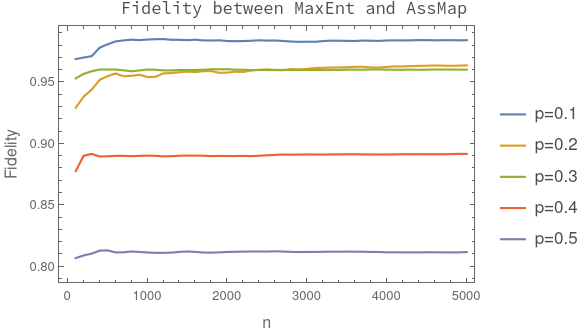
\includegraphics[width=0.6\linewidth]{general/figures/fidelityMaxEntAssMap_vs_n.png}
    \caption{Fidelidad entre el estado de máxima entropía y el estado asignado por promedio como función del número de estados usados en el promedio, para diferentes valores del parámetro $p$.}
    \label{fig:FidMaxEntAssMapN}
\end{figure}
La figura \ref{fig:FidMaxEntAssMapN} muestra que la fidelidad entre ambos estados parece constante siempre que $n>1000$, y que la verdadera dependencia se halla sobre el parámetro $p$. Veamos, pues, la fidelidad entre ambos estados como función de $p$, con $n=1000$.
\begin{figure}[h!]
    \centering
    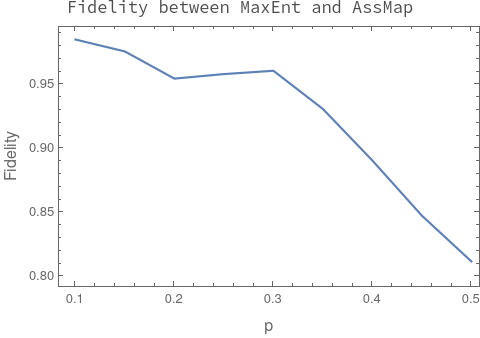
\includegraphics[width=0.6\linewidth]{general/figures/fidelityMaxEntAssMap_vs_p.png}
    \caption{Fidelidad entre el estado de máxima entropía y el estado asignado por promedio como función de $p$.}
    \label{fig:FidMaxEntAssMapP}
\end{figure}
La figura \ref{fig:FidMaxEntAssMapP} es algo burda, y puede que requiera más puntos y observaciones, pero parece revelar que los estados tienden a ser el mismo cuando $p\rightarrow 0,1$. Asumo aquí simetría respecto a $p=0.5$. \notaAd{Bastará con generar puntos entre 0.5 y 1}.
\newpage


\chapter{Resultados para el estado de máxima entropía}

\section{El estado de máxima entropía en términos de $r_{z}$}

La forma matricial de este estado es:
\begin{equation*}
\left(
\begin{array}{cccc}
 \frac{1}{4} e^{-\lambda_{3}} \text{sech}(\lambda_{3} p)
   \text{sech}(\lambda_{3}-\lambda_{3} p) & 0 & 0 & 0 \\
 0 & \frac{e^{2 \lambda_{3}}}{\left(e^{2 \lambda_{3}
   p}+1\right) \left(e^{2 \lambda_{3}}+e^{2 \lambda_{3}
   p}\right)} & 0 & 0 \\
 0 & 0 & \frac{1}{\left(e^{2 \lambda_{3}}+1\right) e^{-2
   \lambda_{3} p}+e^{2 \lambda_{3}-4 \lambda_{3}
   p}+1} & 0 \\
 0 & 0 & 0 & \frac{1}{4} e^{\lambda_{3}}
   \text{sech}(\lambda_{3} p) \text{sech}(\lambda_{3}-\lambda_{3} p) \\
\end{array}
\right)
\end{equation*}
Hallar el valor de $\lambda_{
3}$ en términos del valor $r_{z}$ implica resolver la ecuación:
\begin{equation}\label{eq:RZ}
rz=-\frac{1}{2}\frac{\sinh(\lambda_{3})+(1-2p)\sinh((1-2p)\lambda_{3})}{\cosh(p\lambda_{3})\cosh((1-p)\lambda_{3})}
\end{equation}
No se ve ninguna forma sencilla de despejar al multiplicador de Lagrange. En realidad, esto solo se puede si la función $r_{z}(\lambda_{3})$ tiene inversa, y esto puede depender del parámetro $p$. Graficar la superficie (Figura \ref{fig:rzsurf}) puede aclarar algo el panorama.
\begin{figure}[h!]
\centering
\begin{subfigure}{0.475\textwidth}
  \centering
  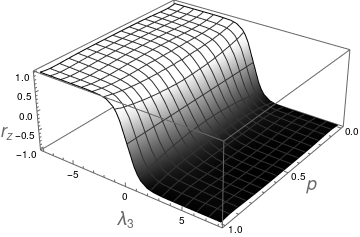
\includegraphics[width=0.6\linewidth]{maxent/figures/LagrangeMult_lambda-8to8.png}
  \caption{$-8<\lambda_{3}<8$}
\end{subfigure}%
\begin{subfigure}{0.475\textwidth}
  \centering
  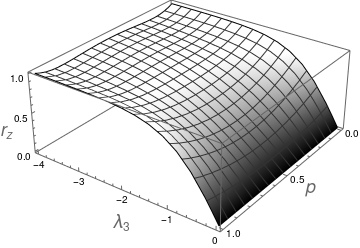
\includegraphics[width=0.6\linewidth]{maxent/figures/LagrangeMult_lambda-4to0.png}
  \caption{$-4<\lambda_{3}<0$}
\end{subfigure}
\caption{Superficie de $r_{z}$ según (\ref{eq:RZ}) para dos intervalos de $\lambda_{3}$. A valores $\lambda_{3}<0$ corresponden valores $r_{z}>0$ y viceversa.}
\label{fig:rzsurf}
\end{figure}

Después de una breve inspección se concluyen las siguientes cosas:
\begin{itemize}
\item la superficie es simétrica respecto al plano $p=0.5$
\item la superficie es antisimétrica  respecto al plano $\lambda_{3}=0$ i.e. $r_{z
}(\lambda_{3},p)=-r_{z
}(-´\lambda_{3},p)$
\item $\text{sgn}(\lambda_{3})=-\text{sgn}(r_{z})$
\end{itemize}

La simetría respecto al plano $p=0.5$ suguiere un cambio de variable $q=\abs{p-0.5}$. La ecuación (\ref{eq:RZ}) se reescribe como:
\begin{equation}\label{eq:RZq}
r_{z}=-\frac{1}{2}\frac{\sinh(\lambda_{3})+2q\sinh(2q\lambda_{3})}{\cosh((q+\frac{1}{2})\lambda_{3})\cosh((q-\frac{1}{2})\lambda_{3})}
\end{equation}
Y nos limitamos al dominio $\lambda_{3}\leq0$ y $0\leq q\leq\frac{1}{2}$. Podemos graficar la función (\ref{eq:RZq}) para diferentes valores de $q$ (Figura \ref{fig:rzinv}).
\begin{figure}[h!]
\centering
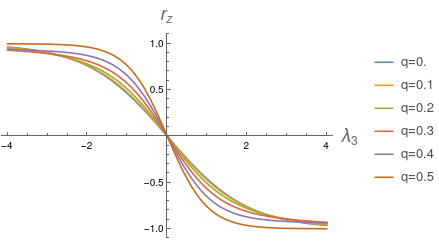
\includegraphics[width=0.6\linewidth]{maxent/figures/rz_has_inverse_lambda-4to4.png}
\caption{$r_{z}$ como función de $\lambda_{3}$ para diferentes valores de $q$. La apariencia uno a uno sugiere la existencia de una inversa.}
\label{fig:rzinv}
\end{figure}

\subsection{Dos soluciones particulares}

Considerando el caso $q=\frac{1}{2}$, la ecuación (\ref{eq:RZq}) se reduce a 
\begin{equation}
r_z=-\frac{1}{2}\frac{2\sinh(\lambda_{3})}{\cosh(\lambda_{3})}
\end{equation}
de manera que $\lambda_{3}=-\text{arctanh}(rz)$.

Si $q=0$, la ecuación (\ref{eq:RZq}) se reduce a
\begin{equation}
r_z=-\frac{\sinh(\lambda_{3})}{\cosh(\lambda_{3}+1)}
\end{equation}
Mathematica sugiere la solución:
\begin{equation}\label{eq:lambda0.5}
\lambda_{3}=\log\qty(\frac{1-r_{z}}{1+r_{z}}).
\end{equation}
\section{La dinámica analítica para el caso $\mcU=\textsc{SWAP}$}

Si se escribe $Z=\Tr{\exp(\lambda_{2}\hat{G}_{3})}$, el estado de máxima entropía compatible con $\rho$ es
\begin{equation}
\varrho_{max}=\frac{1}{Z}\begin{pmatrix}
 e^{-\lambda } & 0 & 0 & 0 \\
 0 & e^{-\lambda  (2 p-1)} & 0 & 0 \\
 0 & 0 & e^{\lambda  (2 p-1)} & 0 \\
 0 & 0 & 0 & e^{\lambda } \\
\end{pmatrix}.
\end{equation}
Este operador de densidad es separable. Es decir, tiene la forma $\varrho_{max}=\varrho_{max}^{A}\otimes\varrho_{max}^{B}$.

Si se aplica el mapeo de grano gureso a este estado, el resultado es precisamente, $\rho$. Si se deja esto en términos de $\lambda_{3}$:
\begin{equation}
\rho(0)=\CG{\varrho_{max}}=\frac{1}{Z}\begin{pmatrix}
 e^{-\lambda }+(1-p)e^{\lambda  (2 p-1)}+p e^{-\lambda  (2 p-1)} & 0 \\
 0 & e^{\lambda }+p e^{\lambda  (2 p-1)}+(1-p)e^{-\lambda  (2 p-1)} \\
\end{pmatrix}.
\end{equation}
El resultado de la dinámica efectiva se puede calcular de forma directa, y es
\begin{equation}
\rho(t=1)=\frac{1}{Z}\CG{S\varrho_{z} S}=
\begin{pmatrix}
 e^{-\lambda }+p e^{\lambda  (2 p-1)}+(1-p) e^{-\lambda  (2 p-1)} & 0 \\
 0 & e^{\lambda }+p e^{-\lambda  (2 p-1)}+(1-p)e^{\lambda  (2 p-1)} \\
\end{pmatrix}
\end{equation}

\subsection{Caso $p=\frac{1}{2}$}

Dentro del estado de máxima entropía, los exponentes de los elementos no extremos de la diagonal se anulan. El resultado es
\begin{equation}
\varrho_{max}=\frac{1}{Z}
\begin{pmatrix}
 e^{-\lambda } & 0 & 0 & 0 \\
 0 & 1. & 0 & 0 \\
 0 & 0 & 1. & 0 \\
 0 & 0 & 0 & e^{\lambda } \\
\end{pmatrix}.
\end{equation}
Usando este, se obtienen tanto el estado efectivo inicial como el estado efectivo final, ambos en términos del multiplicador de Lagrange, y son
\begin{align}
\rho(0)=\CG{\varrho_{max}}=\frac{1}{Z}
\begin{pmatrix}
 1.\, +e^{-\lambda } & 0 \\
 0 & 1.\, +e^{\lambda } \\
\end{pmatrix}, && \rho(1)=\CG{S\varrho_{max} S}=\frac{1}{Z}
\begin{pmatrix}
 1.\, +e^{-\lambda } & 0 \\
 0 & 1.\, +e^{\lambda } \\
\end{pmatrix}.
\end{align}
Si se usa (\ref{eq:lambda0.5}) se halla:
\begin{equation}
\varrho_{max}=\frac{1}{Z}
\begin{pmatrix}
 \frac{1}{4} \left(r_z+1\right){}^2 & 0 & 0 & 0 \\
 0 & \frac{1}{4} \left(1-r_z^2\right) & 0 & 0 \\
 0 & 0 & \frac{1}{4} \left(1-r_z^2\right) & 0 \\
 0 & 0 & 0 & \frac{1}{4} \left(r_z-1\right){}^2 \\
\end{pmatrix}.
\end{equation}
Y recuperamos los estados inicial y final esperados:
\begin{align}
\rho(0)=\CG{\varrho_{max}}=\frac{1}{Z}\begin{pmatrix}
 \frac{1}{2} \left(r_z+1\right) & 0 \\
 0 & \frac{1}{2} \left(1-r_z\right) \\
\end{pmatrix}, && \rho(1)=\frac{1}{Z}\CG{S\varrho_{max} S}=
\begin{pmatrix}
 \frac{1}{2} \left(r_z+1\right) & 0 \\
 0 & \frac{1}{2} \left(1-r_z\right) \\
\end{pmatrix}.
\end{align}

\newpage

\chapter{Resultados para el mapeo de asignación}

\section{Parte analítica}


\subsection{SWAP}
\subsubsection{Estado fino compatible arbitrario}
Sea $\rho\in\mcL(\mcH_{2})$ un estado grueso sobre z definido como en (\ref{eq:rhoz}) y $\varrho$ un estado fino compatible con parametrización de Bloch $\vec{\gamma}$. Sabemos que la acción del coarse graining sobre $\varrho$ es
\begin{equation}\label{eq:CGSWAPprei}
\CG{\varrho}=\frac{1}{2}\qty(\Id+\sum_{k=1}^{3}(p\gamma_{k,0}+(1-p)\gamma_{0,k})\sigma_{k}).
\end{equation}
Este estado, claro, debe estar alineado con el eje $z$, así que se cumple que $p\gamma_{k,0}+(1-p)\gamma_{0,k}=0$ para $k=1,2$. De esta forma, el estado queda como
\begin{equation}\label{eq:CGSWAPi}
\CG{\varrho}=\frac{1}{2}\qty(\Id+(p\gamma_{3,0}+(1-p)\gamma_{0,3})\sigma_{z}).
\end{equation}
Luego, si se aplica el SWAP, el estado grueso efectivo es
\begin{equation}\label{eq:CGSWAPfi}
\CG{S\varrho S}=\frac{1}{2}\qty(\Id+\sum_{k=1}^{3}(p\gamma_{0,k}+(1-p)\gamma_{k,0})\sigma_{k}).
\end{equation}
Para que las ecuaciones (\ref{eq:CGSWAPi}) y (\ref{eq:CGSWAPfi}) correspondan al mismo estado (esto es, que la dinámica efectiva sea la identidad), primero debe de cumplirse que $p\gamma_{0,k}+(1-p)\gamma_{k,0}=0$ para $k=1,2$. Si se combinan ambas condiciones sobre estas componentes se obtiene
\begin{align*}
(2p-1)(\gamma_{k,0}-\gamma_{0,k})&=0,\\
\gamma_{k,0}+\gamma_{0,k}&=0.
\end{align*}
Esto asegura que el estado descrito por (\ref{eq:CGSWAPfi}) esté sobre el eje z, pero para que la coordenada en dicho eje no cambie tras el SWAP subyacente debe cumplirse que 
\begin{equation*}
(2p-1)(\gamma_{3,0}-\gamma_{0,3})=0,
\end{equation*}
De esta forma, puede verse que un estado $\psi$ que cumpla que $\gamma_{k,0}=\gamma_{0,k}=0$ para $k=1,2$ y que $\gamma_{3,0}=\gamma_{0,3}$ no se ve afectado por el SWAP de forma efectiva. Esta invarianza es completamente dependiente del estado fino inicial (o del estado grueso inicial), y las condiciones sobre las componentes se cumplen \notaAd{solo si, estoy seguro de que si se revisan las constantes de estructura sí sale el solo si} si $\rho_{z}$ es puro, y por consiguiente $\varrho=\rho_{z}\otimes\rho_{z}$.

Además, la dinámica efectiva es la identidad siempre que $p=0.5$. Para dicho valor de $p$ se satisfacen todas las condiciones.

\subsubsection{Mapeo de asignación}

Sea $\{\varrho^{j}\}_{j=1}^{N}$ el conjunto usado en el mapeo de asignación, y $\{\vec{\gamma}^{j}\}_{j=1}^{N}$ el conjunto de sus parametrizaciones de Bloch. En tal caso los estados efectivos inicial y final son:
\begin{align}
\rho&=\frac{\sigma_{z}}{N}\sum_{j}(p\gamma_{3,0}^{j}+(1-p)\gamma_{0,3}^{j}),\\
\rho'&=\frac{\sigma_{z}}{N}\sum_{j}(p\gamma_{0,3}^{j}+(1-p)\gamma_{3,0}^{j}).
\end{align}
La dinámica efectiva vuelve a ser la identidad si $p=0.5$ o si $\rho_{z}$ es puro


\newpage


\section{Parte numérica}
\subsection{Cascarón de estados mixtos}
Se generan estados puros $\begin{pmatrix}
a\\
b\\ \end{pmatrix}$ de manera uniforme. Estos son puntos en el cascarón unitario. Todos estos puntos se deplazan radialmente hacia adentro mediante un factor:
\begin{equation}
\vec{\alpha}=r\vec{\alpha_{0}}
\end{equation}
El resultado es un conjunto de estados mixtos $\{\rho_{i}\}_{i=1}^{N}$ cuyos vectores de Bloch se encuentran en el cascarón de radio $r$.

\subsubsection{Mapeo de asignación para el cascarón}


A cada $\rho_{i}$ hay que hallarle su estado fino asignado. Lo que se hace es generar un conjunto $\{\psi_{i}\}_{i=1}^{N}$ de estados finos para un estado grueso en $z$, $\rho_{z}$, tal que su coordenada en $z$ es justamente el radio del cascarón.

Como existe una unitaria $U_{i}$ entre $\rho_{z}$ y cada estado de $\{\rho_{i}\}_{i=1}^{N}$. Entonces podemos aplicar estas unitarias para hallar todos los $\mcA[\rho_{i}]$.

\subsection{Resultados}

Dos experimentos. En el primero se utiliza una probabilidad de swap $p=0.5$ (cascarón de radio $r=0.3$). El conjunto no cambia. En el segundo se utiliza una probabilidad de swap $p=0.3$ (cascarón de radio $r=0.8$).

Se grafican dichos cascarones en azul. Se aplica un SWAP a todos los $\mcA[\rho_{i}]$, y se saca el coarse graining. El resultado se grafica en amarillo.

\begin{figure}[h]
\centering
\begin{subfigure}{0.4\textwidth}
  \centering
  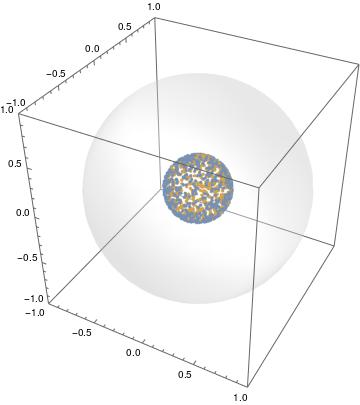
\includegraphics[width=0.8\linewidth]{assmap/figures/effectiveswap_p=0.5_z=0.3.jpeg}
  \caption{$p=0.5$, $r=0.3$, el conjunto no cambia después del swap subyacente}
  \label{fig:paralelogram}
\end{subfigure}
\begin{subfigure}{0.4\textwidth}
  \centering
  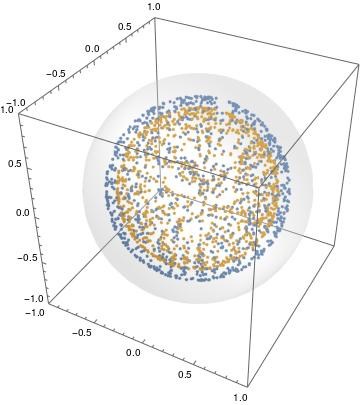
\includegraphics[width=0.8\linewidth]{assmap/figures/effectiveswap_p=0.3_z=0.8.jpeg}
  \caption{$p=0.5$, $r=0.3$, el conjunto se contrae  después del swap subyacente}
  \label{fig:paralelogram}
\end{subfigure}
\label{fig:cooldensities}
\end{figure}

\bibliographystyle{ieeetr}
\bibliography{bibliography}


\end{document}
